\documentclass{article}

\usepackage{arxiv}

\usepackage[utf8]{inputenc} % allow utf-8 input
\usepackage[T1]{fontenc}    % use 8-bit T1 fonts
\usepackage{hyperref}       % hyperlinks
\usepackage{url}            % simple URL typesetting
\usepackage{booktabs}       % professional-quality tables
\usepackage{amsfonts}       % blackboard math symbols
\usepackage{nicefrac}       % compact symbols for 1/2, etc.
\usepackage{microtype}      % microtypography
\usepackage{amsmath}
\usepackage{cleveref}       % smart cross-referencing
\usepackage{graphicx}
\usepackage[super,comma,numbers]{natbib}
\usepackage{doi}
\usepackage{wrapfig}
\usepackage{caption}


\title{ConvPE: Convolutional Position Embedding Improves Transformers}
\date{}
\newif\ifuniqueAffiliation
\uniqueAffiliationtrue
\ifuniqueAffiliation
\author{ {\hspace{1mm}Wang Zehao} \\
	Nanjing University\\
	\texttt{wzhagi@163.com} \\
}
\fi

\begin{document}
\maketitle

\begin{abstract}

ConvPE (Convolutional Position Embedding) substantially improves the performance and efficiency of Transformer models. With only 2.64\% more parameters and a 2.71\% increase in forward-pass time, it reduces training perplexity by 8.41\%. Crucially, it achieves the baseline's final loss with 31.33\% fewer training tokens, yielding a 26.87\% net reduction in wall-clock training time. ConvPE also exhibits superior context extrapolation, reducing validation perplexity by 71.10\% at 4K and 89.84\% at 8K contexts. By generating windowed attention-score biases via a lightweight convolution, ConvPE remains compatible with KV-cache concatenation, various attention masks, and high-dimensional modalities. The code is publicly available at \url{https://github.com/wzhagi/convpe}.

\end{abstract}
\keywords{Position Embedding \and Language Models \and Transformers \and Attention \and Vision Transformers}

\section{Introduction}

\begin{wrapfigure}{r}{0.48\textwidth}
    \centering
    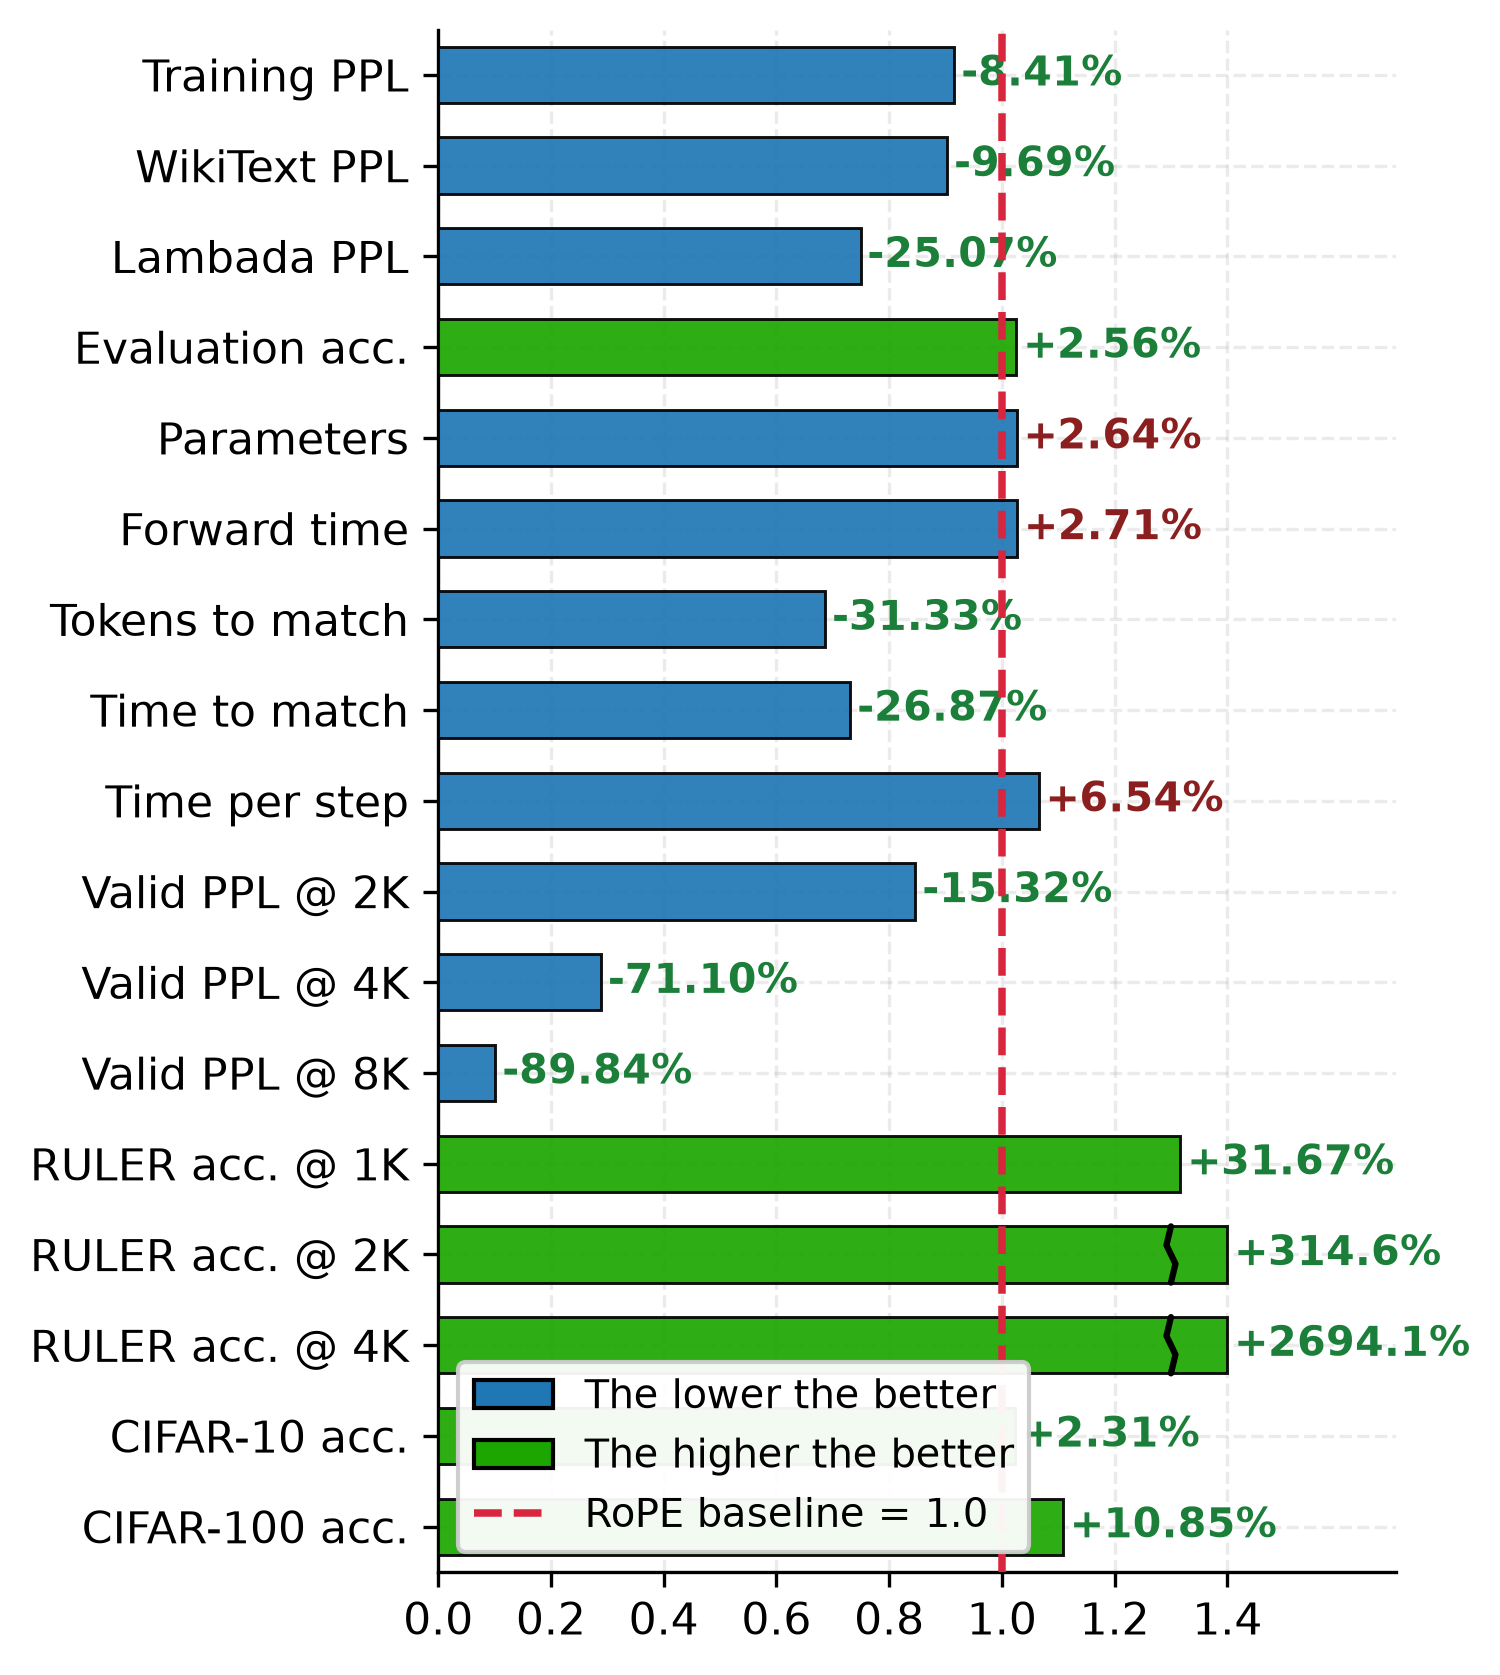
\includegraphics[width=\linewidth]{FIGURES/overview.png}
    \caption{ConvPE / RoPE ratios.}
    \label{fig:overview}
\end{wrapfigure}

Transformers~\cite{vaswani2017attention} are insensitive to input order, whereas word order is crucial for language understanding. Explicit or implicit position embeddings are therefore necessary to inject order information into the model~\cite{devlin2019bert,radford2019language,su2021roformer}.

This paper proposes ConvPE, a simple and efficient position-embedding scheme that generates windowed attention-score biases with a lightweight convolution. This design allows ConvPE to switch freely between different attention masks, be combined with RoPE, support KV-cache concatenation, and naturally extend to high-dimensional modalities with n-dimensional convolution. 

We comprehensively evaluate ConvPE in language-model pretraining and vision transformers. As summarized in Figure~\ref{fig:overview}, ConvPE improves performance and efficiency across the board.

\textbf{Performance:} 

ConvPE reduces training perplexity by 8.41\% and improves average evaluation accuracy by 2.56\%. It also transfers effectively to vision tasks, improving ViT-Tiny~\cite{dosovitskiy2021image} accuracy on CIFAR-10 and CIFAR-100~\cite{krizhevsky2009learning} by 2.31\% and 10.85\%.

\textbf{Training and Token Efficiency:} 

Despite a small 6.54\% per-token wall-clock overhead and 2.64\% more parameters, ConvPE reaches the RoPE baseline's performance with 31.33\% fewer training tokens. This results in a net 26.87\% reduction in total wall-clock training time to match the baseline.

\textbf{Context Extension:} 

ConvPE significantly mitigates performance degradation at zero-shot context extensions. Compared to RoPE, it reduces validation perplexity by 15.32\% at 2K, 71.10\% at 4K, and 89.84\% at 8K. On the RULER benchmark, ConvPE boosts accuracy by 31.67\% at 1K and by over 300\% at 2K and 4K contexts.

\textbf{The main contributions of this paper are as follows:}
\begin{itemize}
    \item We propose ConvPE, a convolutional attention-score-bias position embedding that combines strong performance with broad compatibility.
    \item We study the influence of ConvPE hyperparameters and architecture choices, identifying a simple default configuration with a highly favorable performance--efficiency balance.
    \item We demonstrate that ConvPE significantly improves training efficiency, token efficiency, and zero-shot long-context extrapolation in language models.
    \item We verify the effectiveness of ConvPE2D in vision transformers on CIFAR-10 and CIFAR-100.
    \item We develop high-performance TileLang~\cite{DBLP:journals/corr/abs-2504-17577} kernels for ConvPE.
\end{itemize}

\section{Background}

\subsection{Attention Mechanism}

Given the input query $Q \in \mathbb{R}^{S_q \times D_k}$, key $K \in \mathbb{R}^{S_{kv} \times D_k}$, and value $V \in \mathbb{R}^{S_{kv} \times D_v}$, the computation of scaled dot-product attention~\cite{vaswani2017attention} $O\in \mathbb{R}^{S_q \times D_v}$ is:

$$
O = \mathrm{Attention}(Q,K,V) = \mathrm{softmax}\left(\frac{QK^\top}{\sqrt{d_k}} + \mathbf{B}\right)V
$$

$S_q$ is the query sequence length. $S_{kv}$ is the key/value sequence length. $\mathbf{B}\in\mathbb{R}^{S_q\times S_{kv}}$ is the attention score bias. Causal models introduce a causal mask $M\in\mathbb{R}^{S_q\times S_{kv}}$ that sets the attention score bias $\mathbf{B}$ for invisible positions to $-\infty$. With batch size and multi-head settings, $Q,K,V,O$ additionally have $B,H$ dimensions.

\subsection{Position Embedding}
Existing position embedding schemes can be roughly divided into five categories:

\begin{enumerate}
    \item \textbf{Absolute Position Embedding}~\cite{vaswani2017attention}: adds a fixed positional bias, usually sine waves, to the input vector. It is simple to implement, but its performance is usually limited.
    \item \textbf{Learnable Positional Bias}~\cite{devlin2019bert,radford2019language}: adds a learnable positional bias to the input sequence. It is typically adopted in limited-window settings, such as spatial dimensions in vision models or fixed-rate compression.
    \item \textbf{Rotary Position Embedding}~\cite{su2021roformer}: encodes position as a rotation matrix and applies it to queries and keys, so that attention scores depend on relative positions. RoPE has been widely adopted in modern large language models, enabling long-context extension via frequency scaling, such as YaRN~\cite{peng2024yarn}.
    \item \textbf{Attention Score Bias}: adds a positional bias $B$ to attention scores~\cite{raffel2020exploring,press2021train,chang2021convolutionsselfattentionreinterpretingrelative}. RoPE can be viewed as a rotation-based equivalent, as it also makes attention scores depend on relative positions.
    \item \textbf{No Position Embedding (NoPE)}~\cite{kazemnejad2023impact}: adds no explicit position embeddings; instead, it relies on model structure and causal attention masks to implicitly learn positional information requiring no explicit Position Embedding~\cite{kimi2026k3}.
\end{enumerate}


\section{Method}
Given token representations $X\in\mathbb{R}^{B\times S\times D}$, ConvPE first projects them to a small channel dimension $X_{down}\in\mathbb{R}^{B\times S\times C}$, then uses a convolution to generate windowed attention score bias $\mathbf{B}_{ConvPE}\in\mathbb{R}^{B\times S\times H_b\times W}$ for self-attention keys within the convolution window as shown in Figure~\ref{fig:convpe_method}.

\begin{figure}[!ht]
    \centering
    \begin{minipage}{0.52\textwidth}
        \centering
        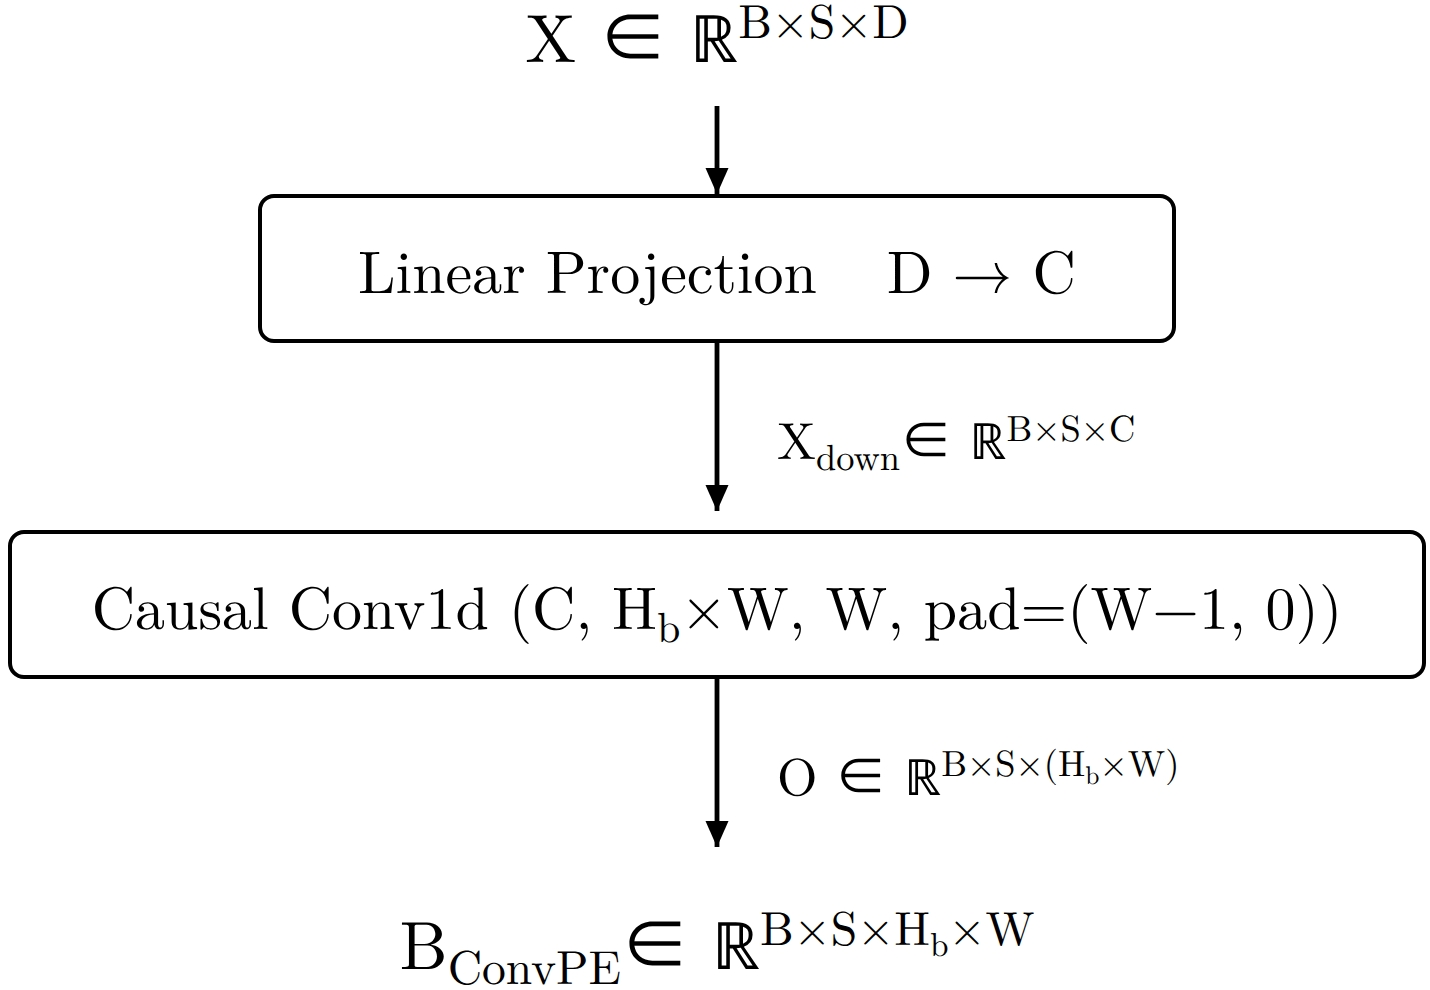
\includegraphics[width=\linewidth]{FIGURES/convpe.jpeg}
    \end{minipage}
    \hfill
    \begin{minipage}{0.38\textwidth}
        \centering
        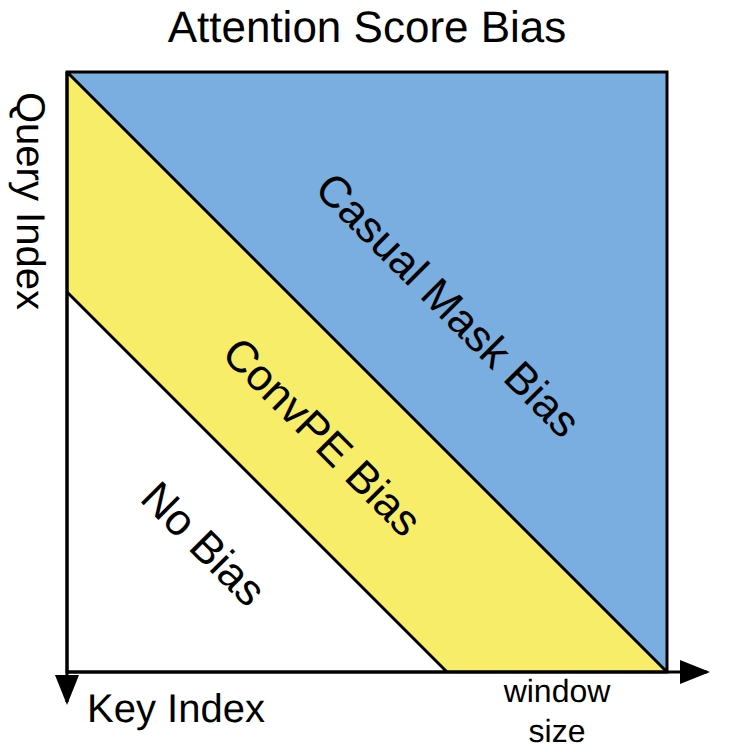
\includegraphics[width=\linewidth]{FIGURES/score_bias.jpeg}
    \end{minipage}
    \caption{ConvPE Algorithm}
    \label{fig:convpe_method}
\end{figure}

\begin{equation*}
\mathbf{B}^{b,h,s_q,s_{kv}}=
\begin{cases}
\mathbf{B}_{\mathrm{ConvPE}}^{b,s_q,h\bmod H_b,w}, & w\in [0,W-1] \text{ where } w=s_{kv}-s_q+W-1\\
0, & \text{otherwise}.
\end{cases}
\end{equation*}


The hyperparameters are:
\begin{itemize}
\item $W$: convolution window size.
\item $C$: out features of linear projection and in channels of convolution.
\item $H_{b}$: number of score bias heads.
\end{itemize}

The convolution takes $C$ input channels, uses a kernel of size $W$, and outputs
$H_b\times W$ channels. The projection has $D\times C$ parameters and
the convolution has $W^2\times C\times H_b$ parameters; the computation (MACs) per token is the same as the parameter count.

To reduce the convolution parameter count, we introduce three additional
hyperparameters:
\begin{itemize}
\item $\mathrm{Groups}$: number of convolution groups;
\item $\mathrm{Share}$: whether to share weights across convolution groups;
\item $\mathrm{Rank}$: rank used in the low-rank convolution.
\end{itemize}


\section{Experiments}
All models in our experiments use Multi-Query Attention (MQA)~\cite{shazeer2019fast}, with $K=V$~\cite{deepseek2026v4}. Each attention layer has $D_{model} \times D_{head} \times (2\times N_{heads}+1)$ parameters. Each feed-forward layer uses SwiGLU~\cite{shazeer2020glu} and has $8\times D_{model}^2$ parameters. 

\subsection{Hyperparameter Search}
We train each model for one epoch on WikiText-103~\cite{merity2016pointer} and record the validation loss. Training uses the Hugging Face Trainer~\cite{wolf2020transformers}, AdamW~\cite{loshchilov2019decoupled}, and the GPT-2 tokenizer~\cite{radford2019language}. The training hyperparameters are: batch size $4$, sequence length $1024$, learning rate $3\times10^{-4}$ with cosine learning-rate scheduler, and seed $42$.

We train two types of backbone models, a tiny backbone with $N_{layers}=12$, $D_{model}=192$, $N_{heads}=3$, $D_{head}=64$, and a base backbone with $N_{layers}=12$, $D_{model}=768$, $N_{heads}=12$, $D_{head}=128$. The model name format is "\texttt{backbone RoPE/NoPE  $W$ $C$ $\mathrm{Rank}$ $H_{b}$ $\mathrm{Groups}$ $\mathrm{Share}$}". For example, "\texttt{tiny rope w128d6r128h3g1s}" denotes a tiny backbone using RoPE with $W=128$, $C=6$, $\mathrm{Rank}=128$, $H_b=3$, $\mathrm{Groups}=1$, and $\mathrm{Share}$ weights. For simplicity, model names may omit the default configuration: \texttt{NoPE}, \texttt{r0}(no low-rank convolution), \texttt{h1} ($H_b=1$), \texttt{g1}($\mathrm{Groups}=1$), and \texttt{s0} (no weight sharing).

\begin{figure}[!ht]
    \centering
    \begin{minipage}{0.48\textwidth}
        \centering
        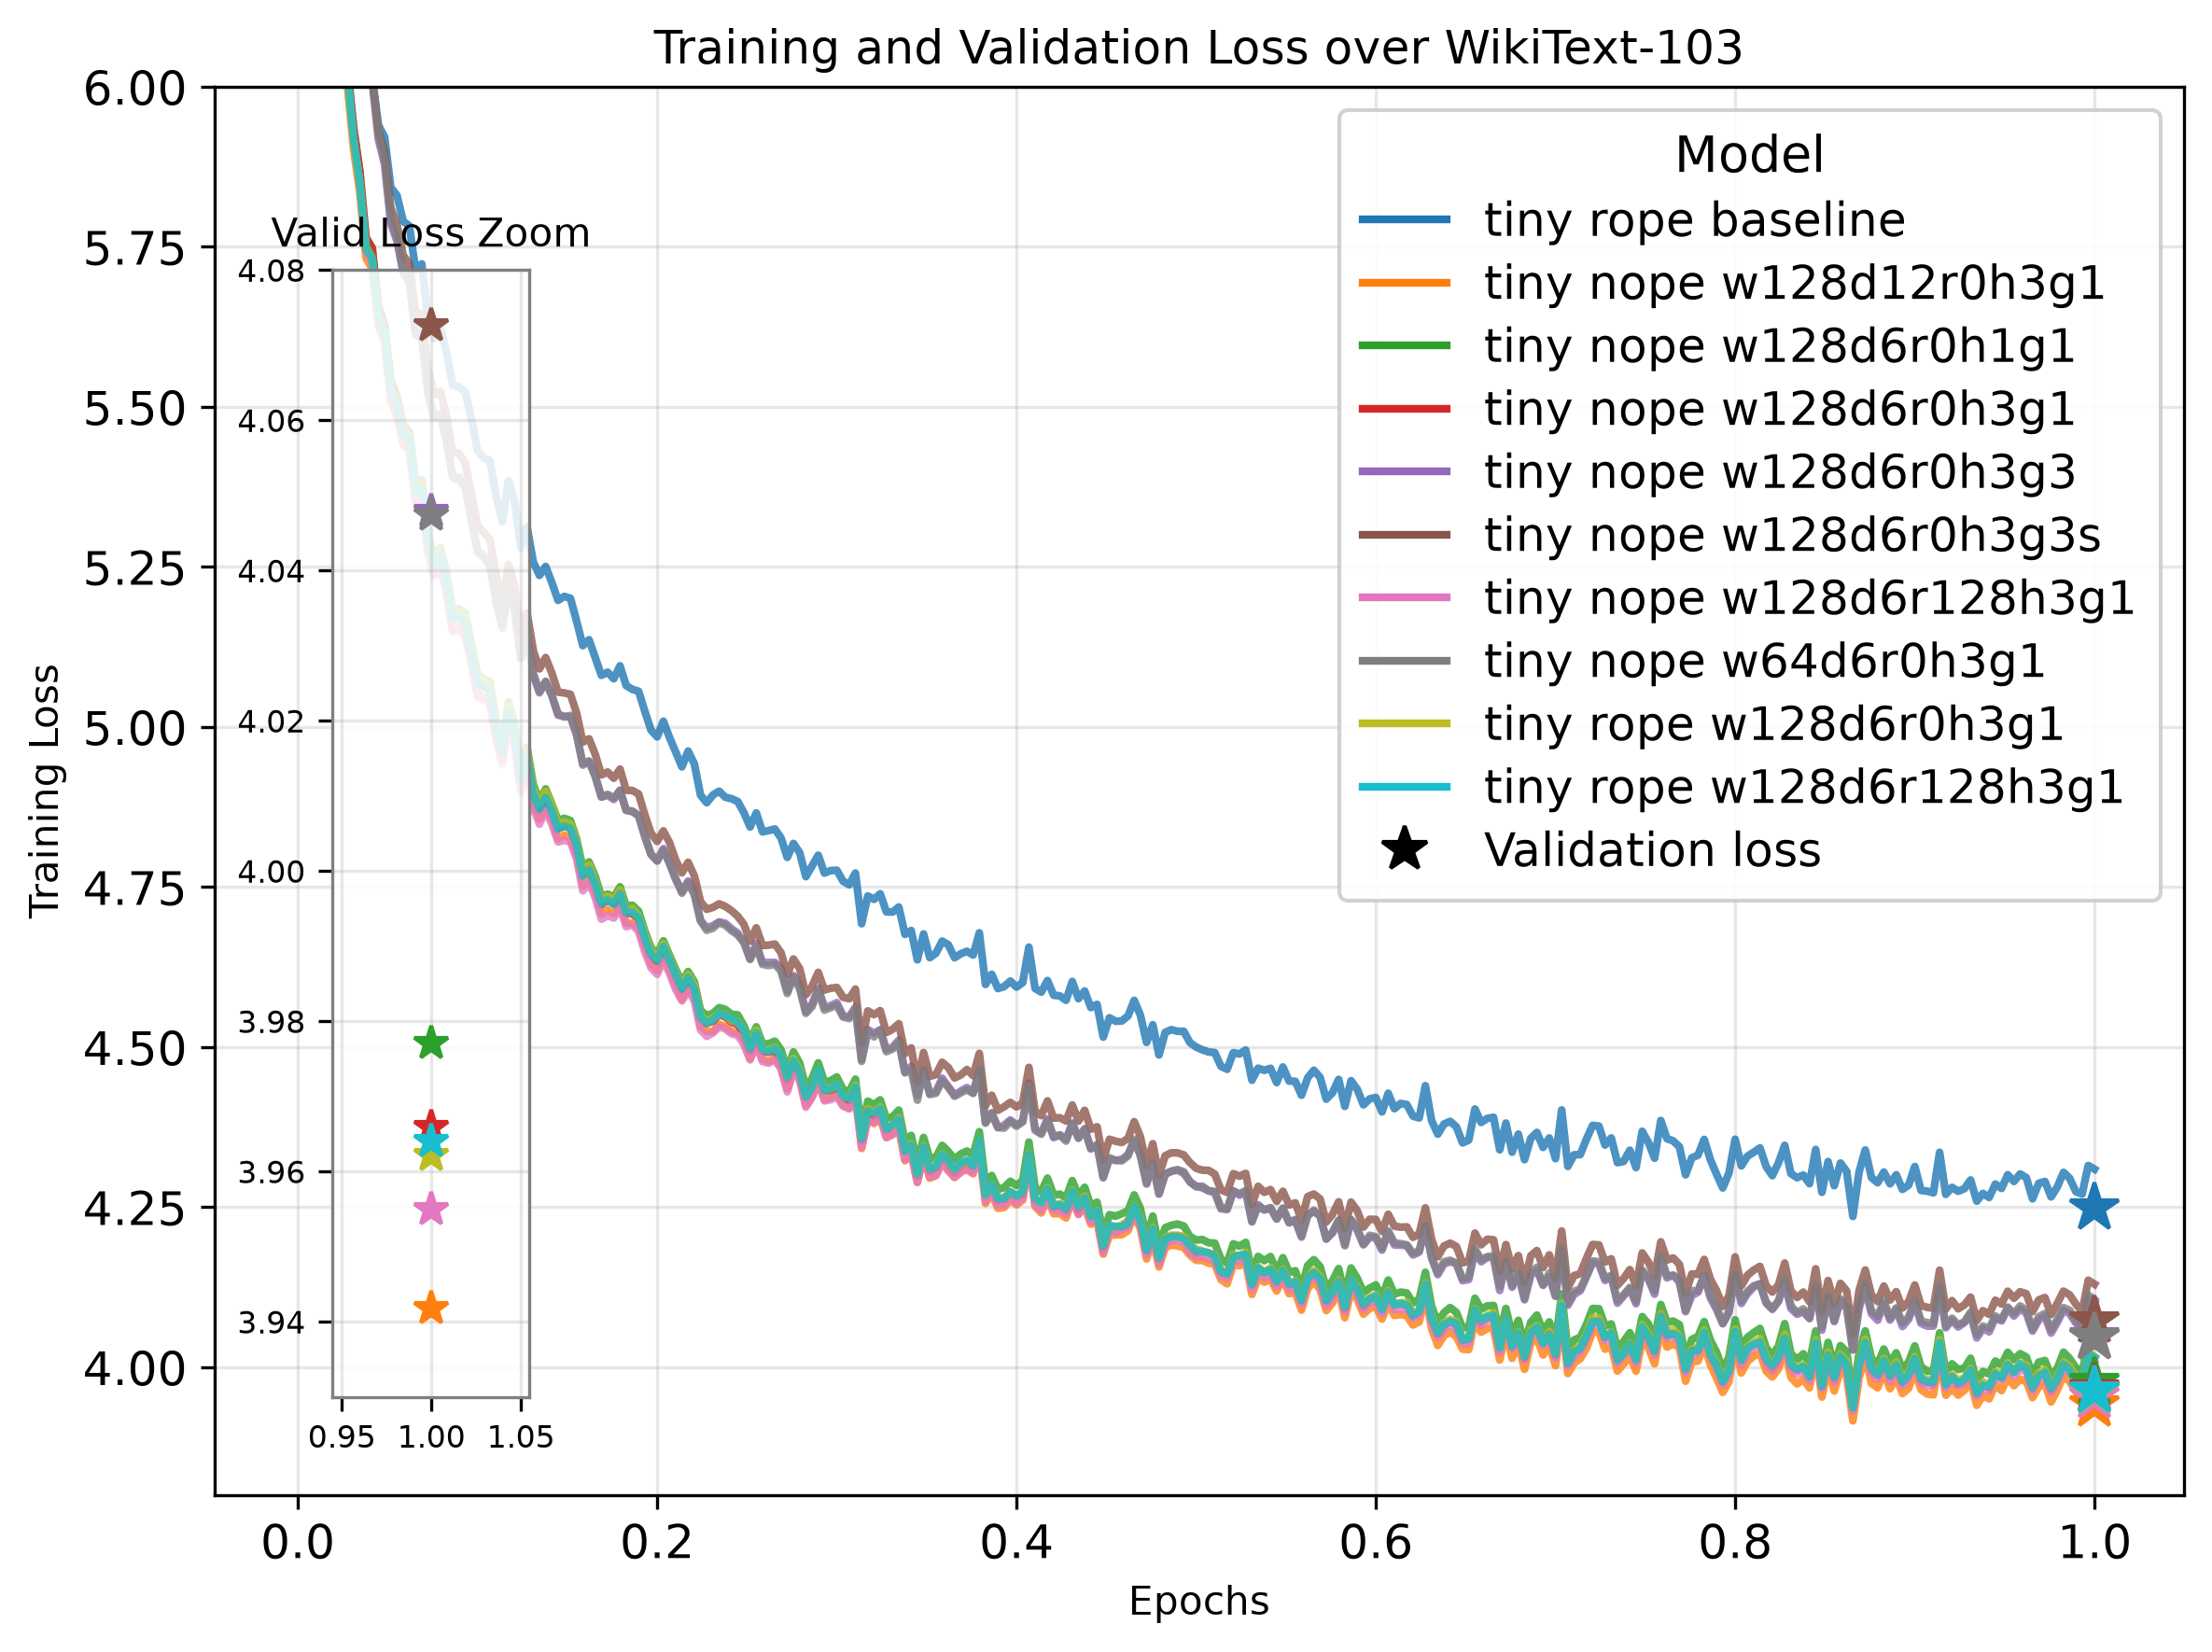
\includegraphics[width=\linewidth]{FIGURES/wikitext103tiny.png}
        \caption{Tiny model training curve on WikiText-103}
        \label{fig:wt103t}
    \end{minipage}
    \hfill
    \begin{minipage}{0.48\textwidth}
        \centering
        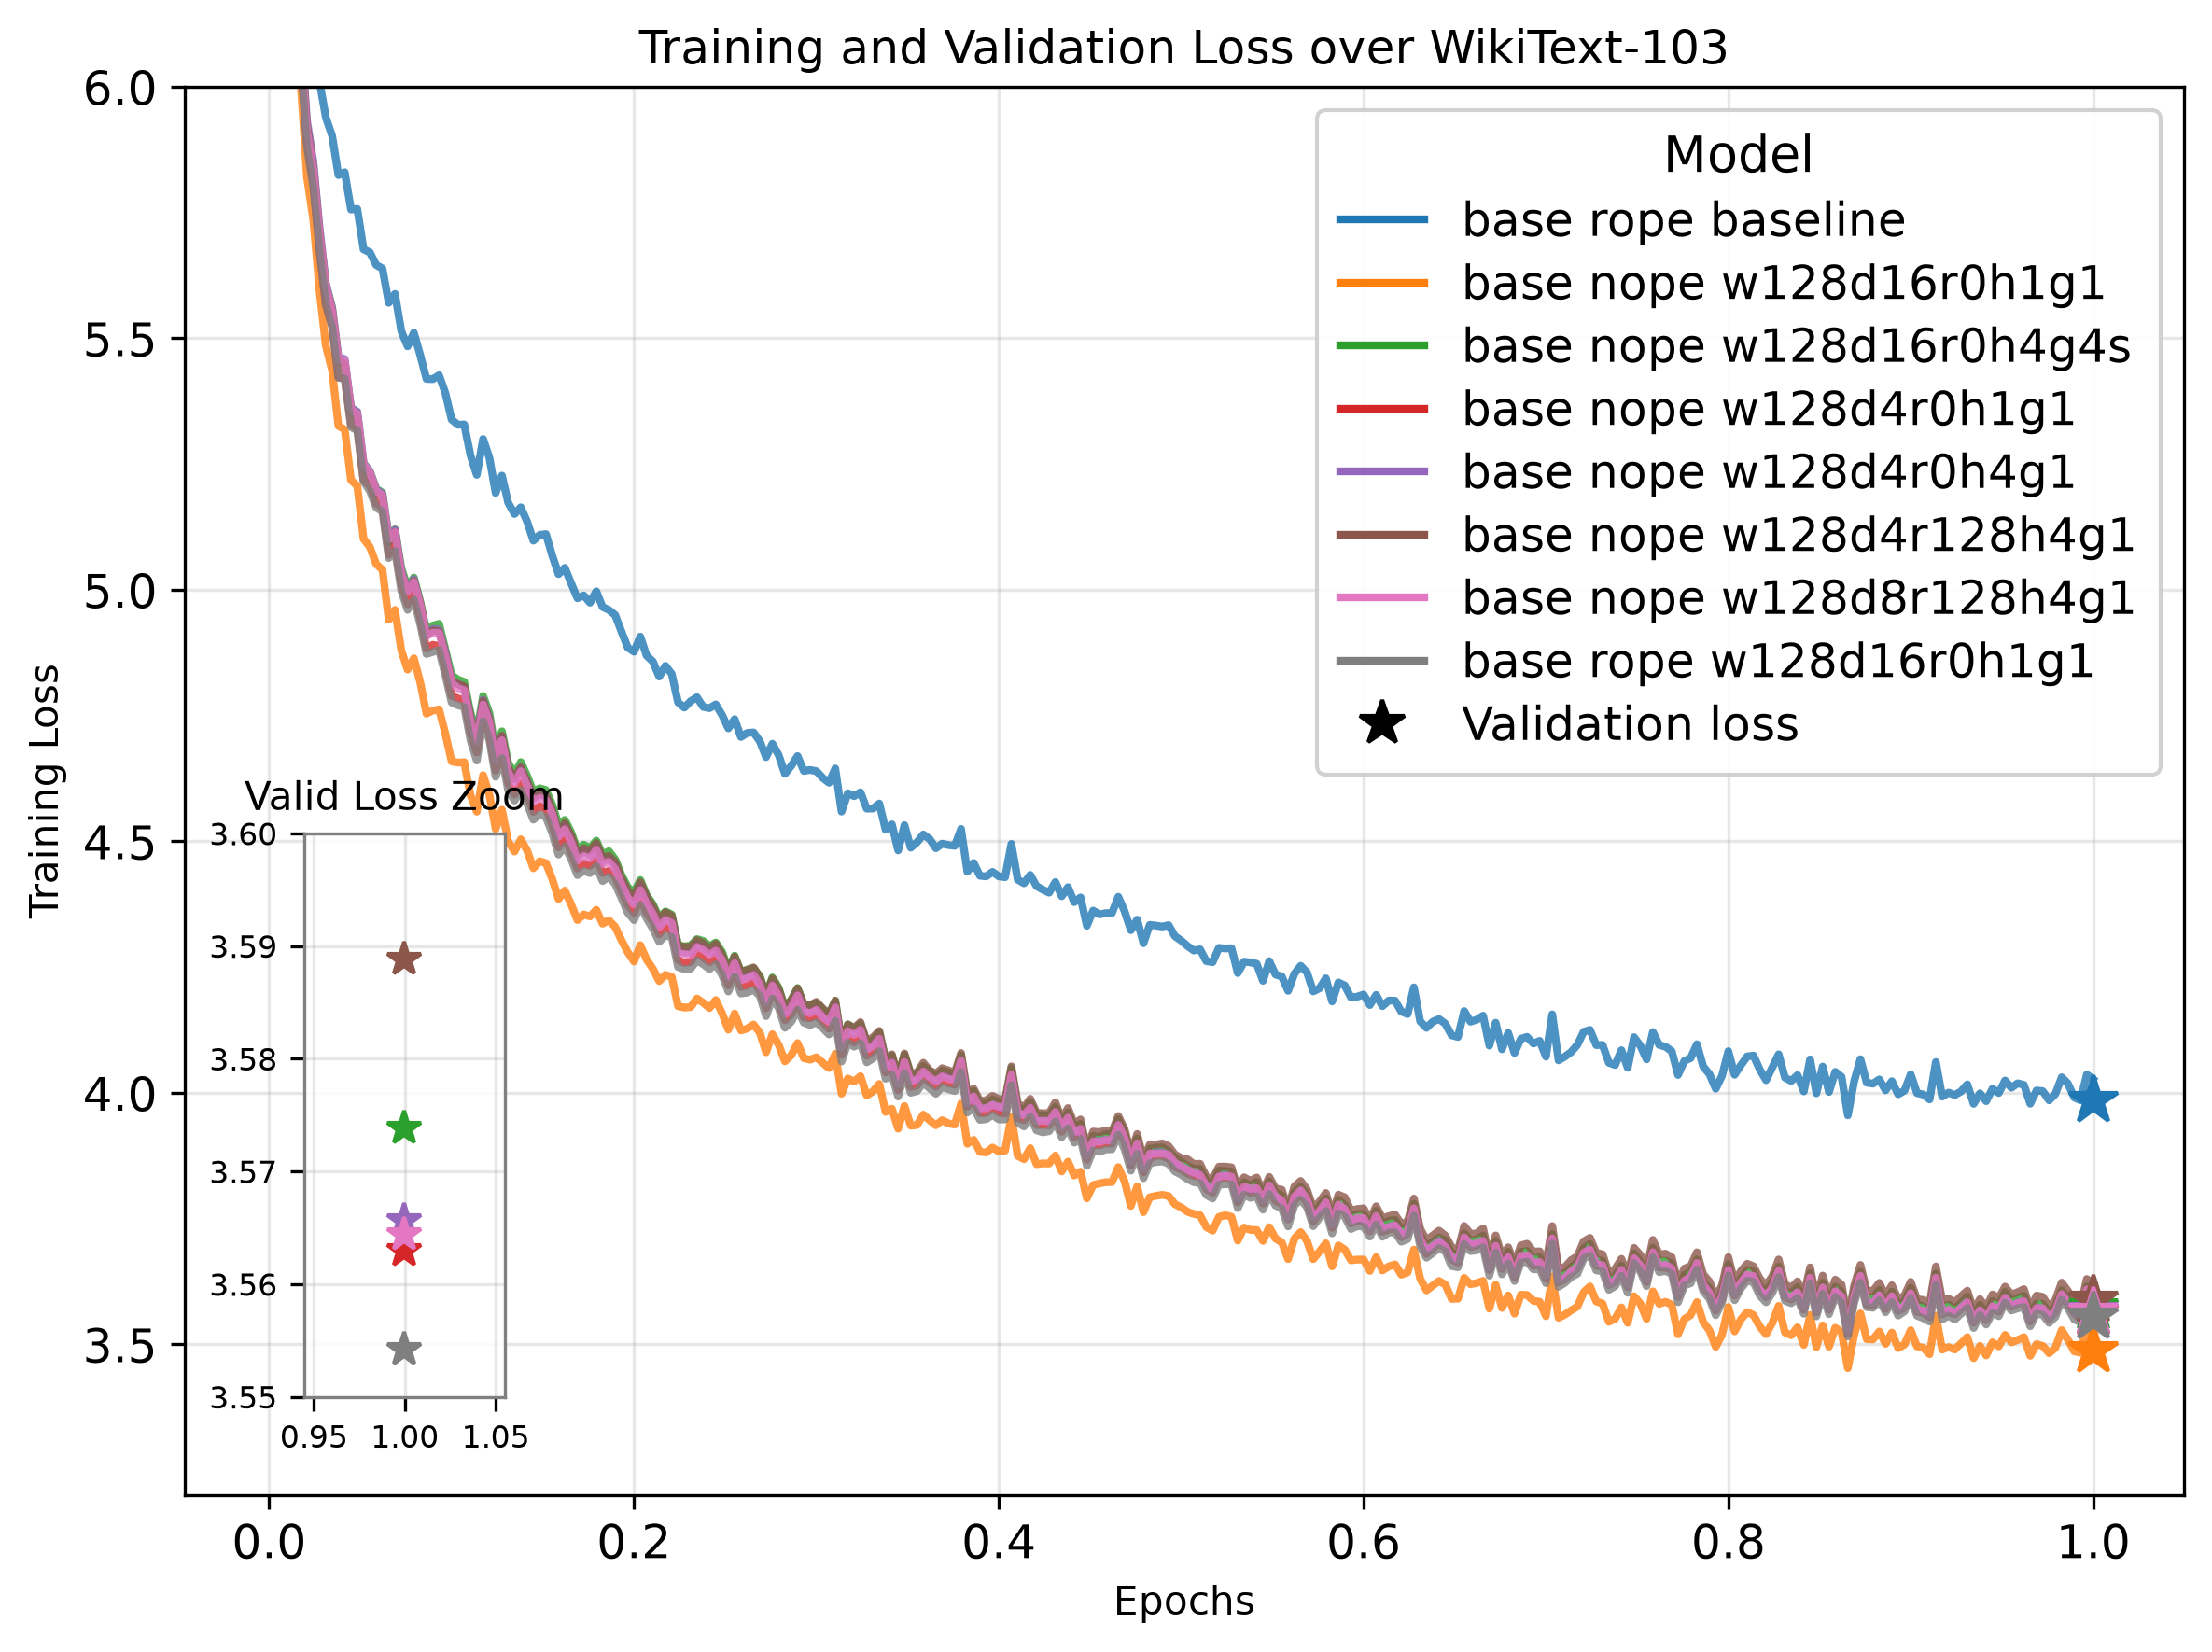
\includegraphics[width=\linewidth]{FIGURES/wikitext103base.png}
        \caption{Base model training curve on WikiText-103}
        \label{fig:wt103b}
    \end{minipage}
\end{figure}

First, we train tiny models with hyperparameters around "\texttt{nope w128d6r0h3g1}". Figure~\ref{fig:wt103t} shows that all ConvPE variants outperform the RoPE baseline. The largest gains come from increasing the window size and the projection dimension. Using grouped convolution causes the largest performance drop. RoPE integration and other parameter-saving methods show minor differences from "\texttt{nope w128d6r0h3g1}".

We then train base models with hyperparameters around "\texttt{nope w128d4r0h4g1}" and "\texttt{nope w128d16r0h1g1}". Figure~\ref{fig:wt103b} shows that $H_b=1$ without any parameter-saving technique achieves the best balance between performance and parameter efficiency.

In additional experiments, we also try using $X$, $Q$~\cite{chang2021convolutionsselfattentionreinterpretingrelative} or $KV$ as the convolution input, but performance drops.

\subsection{Pretraining}

\begin{figure}[!ht]
    \centering
    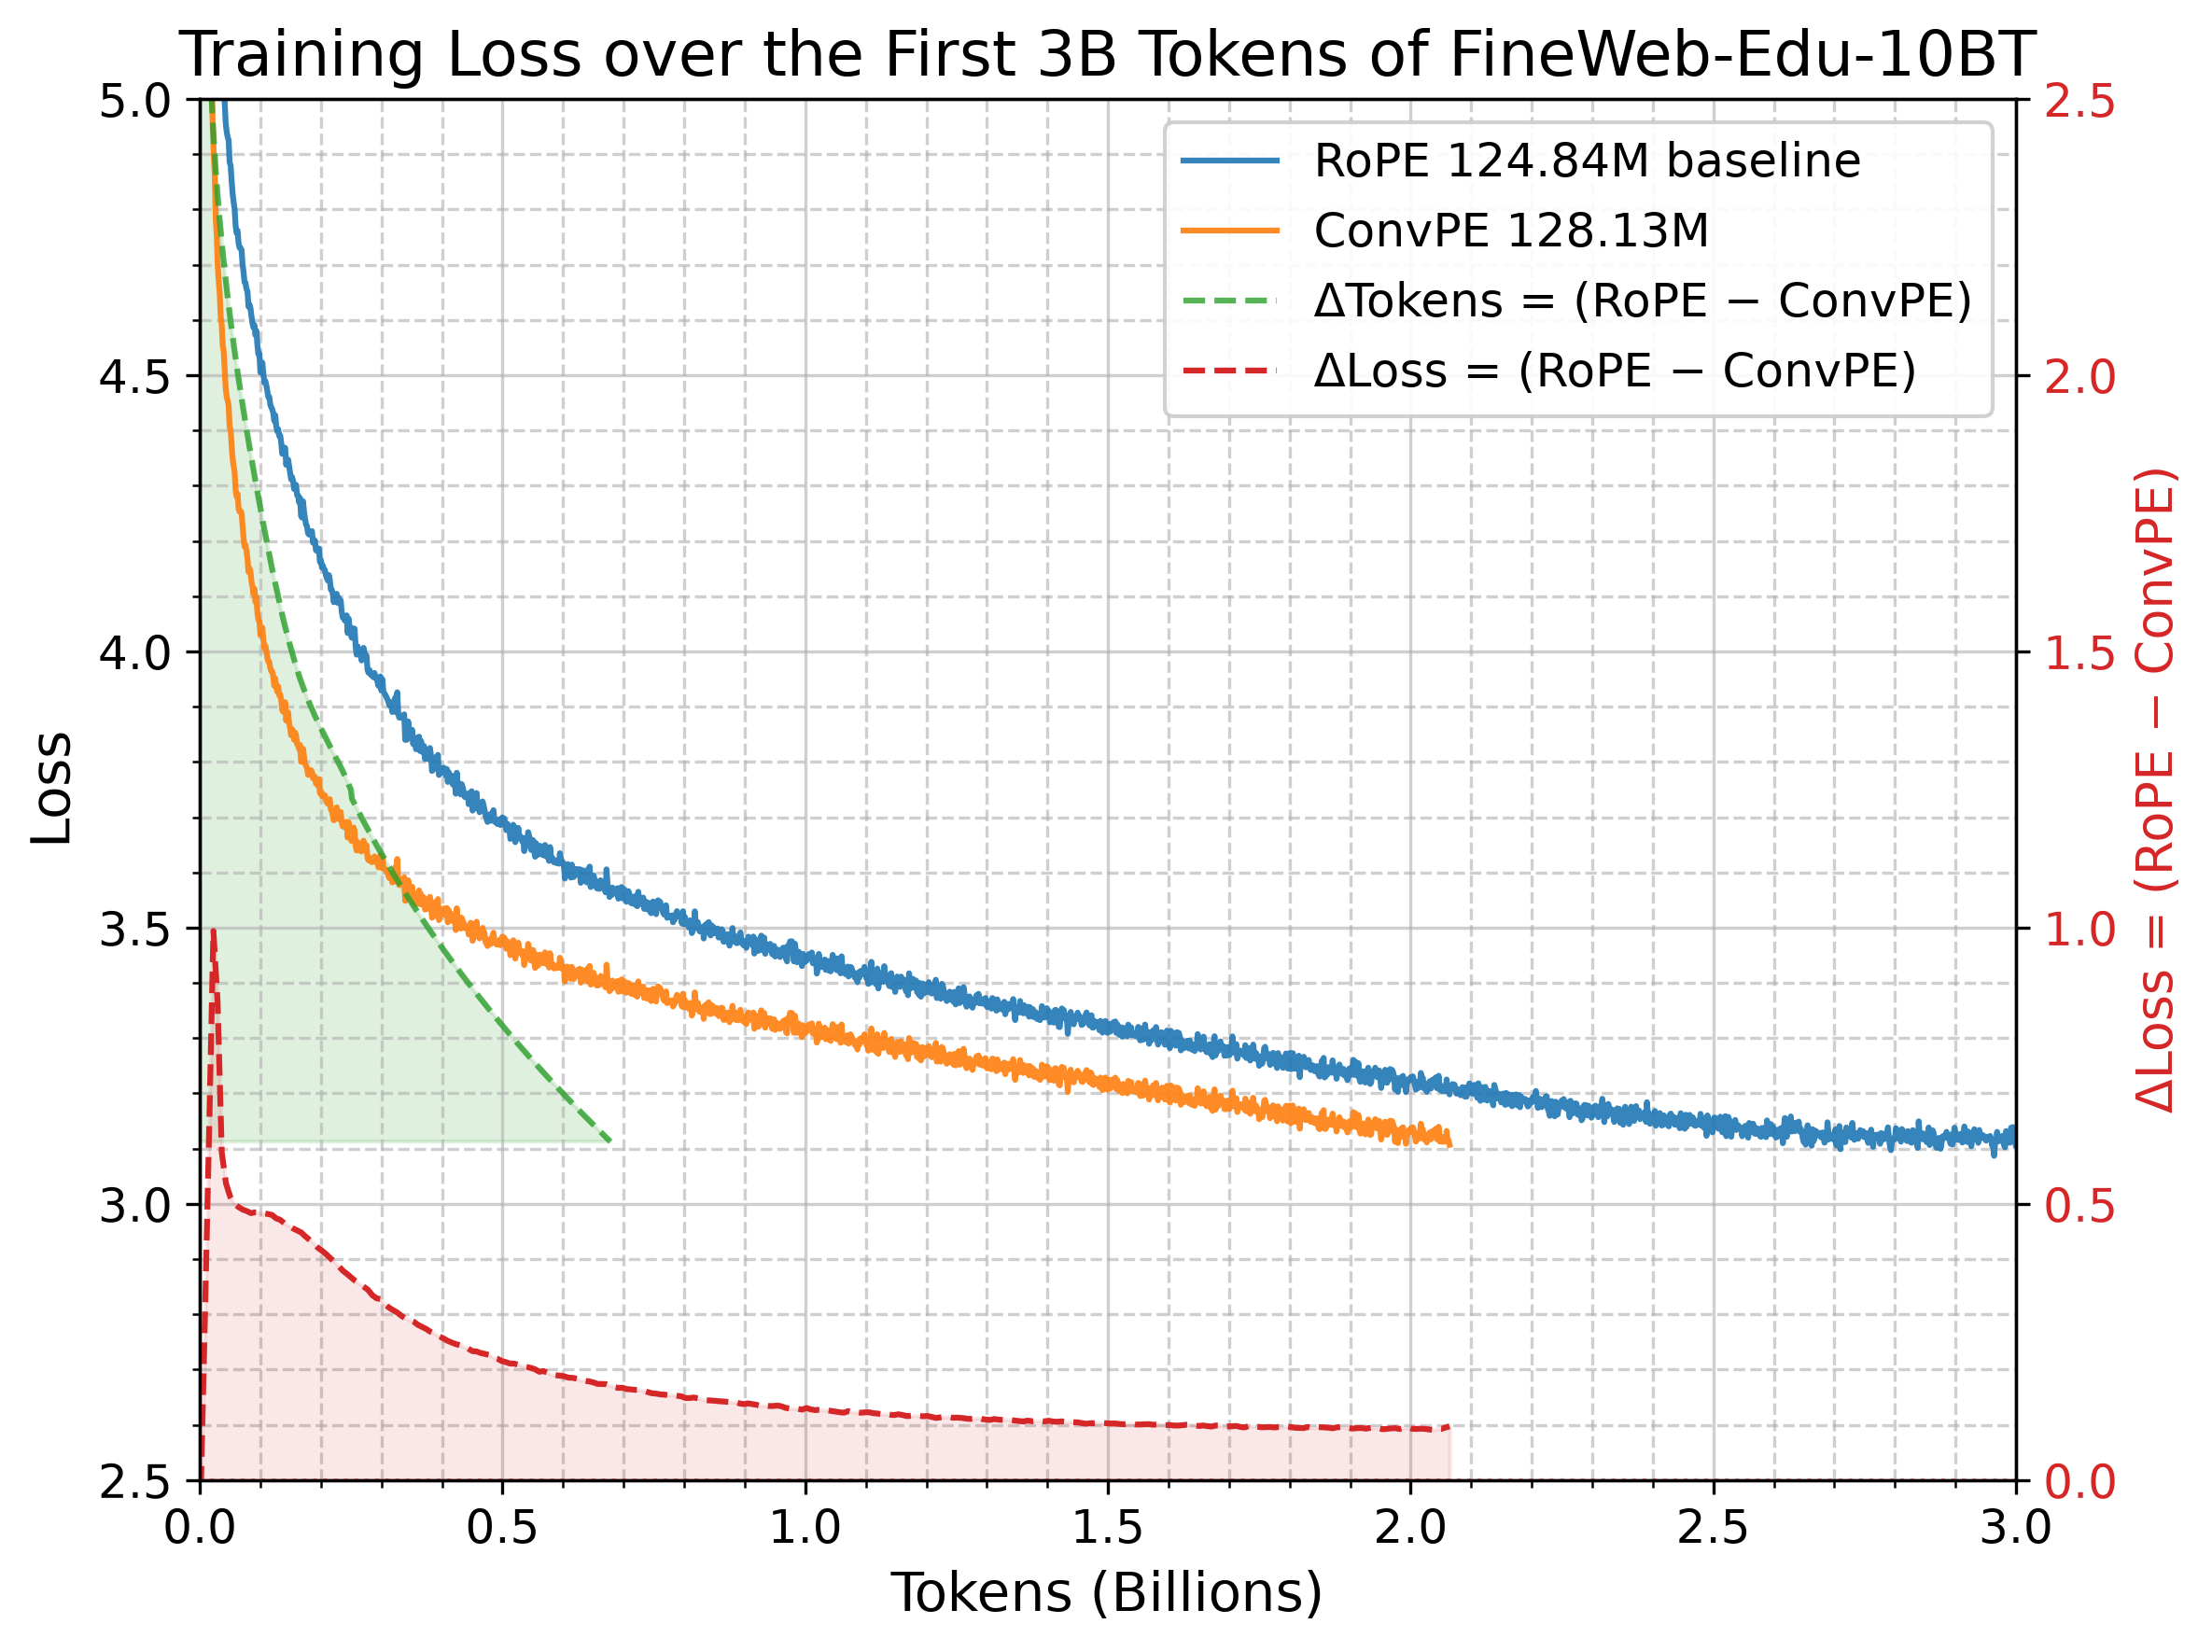
\includegraphics[width=0.8\linewidth]{FIGURES/pretrain.png}
    \caption{Pretraining curve on the first 3B tokens of FineWeb-Edu-10BT}
    \label{fig:pretrain}
\end{figure}

We choose "\texttt{base w128d16}" as the ConvPE variant configuration for performance and throughput considerations. We train the RoPE baseline and the ConvPE variant from scratch on the first 3B tokens of FineWeb-Edu-10BT. We use Muon~\cite{jordan2024muon} to optimize the 2D parameters, excluding the embedding layer and the language head, with a learning rate of $3\times10^{-3}$, while Adam~\cite{DBLP:journals/corr/KingmaB14} optimizes the remaining parameters at a learning rate of $3\times10^{-4}$, both using a cosine learning-rate scheduler. The training hyperparameters are: batch size $4$, gradient accumulation steps $4$, sequence length $1024$, and seed $42$.

Figure~\ref{fig:pretrain} shows that ConvPE converges faster and achieves a lower final loss compared to the RoPE baseline. We implement high-performance Flash MQA kernels
in TileLang and benchmark two configurations: \texttt{base RoPE} with
$124.84$M parameters and \texttt{base w128d16} with $128.13$M parameters
($+2.64\%$), using a batch size of $4$ and a sequence length of $1024$. While the
forward-pass time increases by $2.71\%$, slightly exceeding the parameter increase, the final training loss drops from $3.1195$ to $3.0316$ ($-2.82\%$). According to scaling laws~\cite{kaplan2020scaling,hoffmann2022training}, such a substantial loss reduction would typically require a model with $\sim 50\%$ more parameters. More importantly, despite the $6.54\%$ per-step overhead, the number of training tokens required to match the RoPE baseline's final loss decreases from $3$B to $2.06$B, a $31.33\%$ reduction. This translates to a net reduction in total wall-clock training time of approximately $26.87\%$.

\subsection{Evaluations}
This section evaluates the pretrained ConvPE and the RoPE baseline on pretraining and context-extension benchmarks without any fine-tuning.
\subsubsection{Pretraining Evaluations}

\begin{table}[!ht]
\centering
\begin{tabular}{ccccc}
\toprule
Dataset & Metric & RoPE & ConvPE & Random \\
\midrule
wikitext & perplexity & 46.56 & \textbf{42.05} & - \\
lambada & perplexity, acc & 118.10, 0.2507 & \textbf{88.49}, \textbf{0.2604} & - \\
hellaswag & acc, acc norm & 0.2894, 0.3148 & \textbf{0.2949}, \textbf{0.3272} & 0.25 \\
xstorycloze\_en & acc & 0.5460 & \textbf{0.5526} & 0.5 \\
piqa & acc, acc norm & 0.6251, 0.6208 & \textbf{0.6338}, \textbf{0.6235} & 0.5 \\
arc\_easy & acc, acc norm & 0.5114, 0.4487 & \textbf{0.5421}, \textbf{0.4701} & 0.25 \\
winogrande & acc & 0.5091 & \textbf{0.5193} & 0.5 \\
boolq & acc & 0.5676 & \textbf{0.5893} & 0.5 \\
truthfulqa\_mc1 & acc & 0.2399 & 0.2375 & \textbf{0.25} \\
\bottomrule
\end{tabular}
\captionof{table}{Evaluation results of pretraining models}
\label{tab:pe}
\end{table}

Table~\ref{tab:pe} shows that ConvPE consistently improves language-modeling performance over the RoPE baseline. On WikiText, perplexity drops from 46.56 to 42.05, and on LAMBADA perplexity decreases substantially from 118.10 to 88.49, with accuracy also improving from 0.2507 to 0.2604. ConvPE also outperforms RoPE on most downstream benchmarks. The gains are consistent across most metrics. The main exception is TruthfulQA-MC1, where both models fall below the random-choice baseline, indicating that this benchmark remains difficult for both models. Overall, the pretraining results support ConvPE as a stronger positional encoding than RoPE for the evaluated language tasks.

\begin{table}[!ht]
\centering
\begin{minipage}[c]{0.48\textwidth}
\centering
\begin{tabular}{ccc}
\toprule
Context& RoPE & ConvPE \\
\midrule
1K & 3.1247 & \textbf{3.0312} \\
2K & 3.1684 & \textbf{3.0021} \\
4K & 4.2690 & \textbf{3.0278} \\
8K & 5.6443 & \textbf{3.3575} \\
\bottomrule
\end{tabular}
\captionof{table}{Validation loss on 1M training tokens}
\label{tab:valloss}
  \vspace{1.2em}
    \begin{tabular}{cccc}
        \toprule
        model & params & CIFAR-10 & CIFAR-100 \\
        \midrule
        RoPE baseline    & 5.346M & 0.910 & 0.627 \\
        ConvPE2D \texttt{w3d4}& 5.359M & 0.931 & \textbf{0.695} \\
        ConvPE2D \texttt{w3d8}& 5.372M & \textbf{0.933} & 0.683 \\
        ConvPE2D \texttt{w5d4}& 5.402M & 0.929 & 0.682 \\
        ConvNet & 4.335M & \textbf{0.945} & \textbf{0.737} \\
        \bottomrule
    \end{tabular}
    \captionof{table}{Validation accuracy on CIFAR-10 and CIFAR-100}
    \label{tab:cifar}
\end{minipage}
\hfill
\begin{minipage}[c]{0.48\textwidth}
  \centering
  \begin{tabular}{cccc}
\toprule
Task & Context & RoPE & ConvPE \\
\midrule
niah\_single\_1   & 1K & 0.614 & \textbf{0.890} \\
 & 2K & 0.004 & \textbf{0.722} \\
 & 4K & 0.000 & \textbf{0.314} \\
niah\_single\_2   & 1K & 0.612 & \textbf{0.664} \\
 & 2K & 0.000 & \textbf{0.038} \\
niah\_single\_3   & 1K & 0.090 & \textbf{0.180} \\
 & 2K & 0.000 & \textbf{0.014} \\
niah\_multikey\_1 & 1K & 0.198 & \textbf{0.200} \\
 & 2K & 0.118 & \textbf{0.194} \\
 & 4K & 0.000 & 0.002 \\
niah\_multikey\_2 & 1K & 0.002 & 0.000 \\
niah\_multikey\_3 & 1K & 0.000 & 0.008 \\
niah\_multiquery & 1K & 0.104 & \textbf{0.186}\\
 & 2K & 0.029 & \textbf{0.179} \\
 & 4K & 0.000 & 0.000 \\
niah\_multivalue & 1K & 0.149 & \textbf{0.187} \\
 & 2K & 0.127 & \textbf{0.186} \\
 & 4K & 0.000 & 0.000 \\
ruler\_vt        & 1K & \textbf{0.032} & 0.008 \\
 & 2K & 0.000 & \textbf{0.052} \\
 & 4K & 0.000 & \textbf{0.107} \\
ruler\_cwe       & 1K & 0.002 & 0.002 \\
ruler\_fwe       & 1K & 0.001 & \textbf{0.012} \\
ruler\_qa\_squad  & 1K & 0.148 & \textbf{0.191} \\
 & 2K & 0.078 & \textbf{0.091} \\
 & 4K & 0.017 & \textbf{0.052} \\
\bottomrule
\end{tabular}
\captionof{table}{RULER evaluations}
\label{tab:ruler}
\end{minipage}
\end{table}

\subsubsection{Context Extension Evaluations}

We first evaluate language-modeling performance using 1M tokens from the training dataset with increasing context length. Both models are pretrained on 1K-token contexts. Table~\ref{tab:valloss} shows a clear advantage for ConvPE in language modeling as context length increases. RoPE degrades sharply beyond 2K, whereas ConvPE remains comparatively stable up to 4K and degrades much more gracefully at 8K. This indicates that ConvPE provides better context-length extrapolation and preserves model performance under longer contexts.

We then evaluate both models on RULER tasks. Table~\ref{tab:ruler} shows that ConvPE generally improves over RoPE on several long-context retrieval and reasoning tasks, particularly at 1K and 2K contexts. ConvPE even performs well at 4K contexts on some tasks. Some tasks remain near zero for both models, indicating that these tasks are too difficult for 125M-parameter models. Although the language-modeling loss of ConvPE remains stable up to 4K, the downstream tasks show that zero-shot context extension is still far from solved.


\subsection{2D Position Embedding}

To produce 2D positional embeddings, we use 2D convolutional layers that take
a 2D window input and produce a 2D window output. We use ViT-Tiny~\cite{dosovitskiy2021image} models with Multi-Head Attention (MHA) and the configuration
$N_{\mathrm{layers}}=12$, $D_{\mathrm{model}}=192$, $N_{\mathrm{heads}}=3$, and $D_{\mathrm{head}}=64$. We train the models on CIFAR-10 and CIFAR-100~\cite{krizhevsky2009learning} for 100 epochs with patch shape $4\times 4$.

Table~\ref{tab:cifar} shows that ConvPE transfers effectively to vision transformers and outperforms the RoPE baseline. The influence of hyperparameters requires further study on larger models and datasets.

\section{Conclusions and Future Work}

ConvPE delivers substantial performance gains at a minor parameter and computational cost, providing a powerful alternative for positional embeddings. We adopt $H_b=1$ without any parameter-saving technique as the default configuration, which achieves the best balance among performance, parameter efficiency, and computational cost. ConvPE is compatible with RoPE, various attention masks, and KV-cache concatenation, and it naturally supports multidimensional extensions. 

Future work can explore the following directions:
\begin{itemize}
    \item \textbf{Kernel Optimization.} Further optimize the backward kernel and develop additional kernels for a wider range of hardware.
    \item \textbf{Scaling behavior.} Investigate ConvPE with larger Transformers and datasets, and identify configuration patterns at scale.
    \item \textbf{Long-context modeling.} Evaluate ConvPE in long-context settings, where positional generalization is particularly important.
    \item \textbf{Architectural integration.} Combine ConvPE with Sliding Window Attention (SWA)~\cite{beltagy2020longformer}, Compressed Sparse
    Attention (CSA)~\cite{deepseek2026v4}, and other Transformer variants.
    \item \textbf{Multidimensional modalities.} Extend ConvPE to high-dimensional modalities such as vision, speech, and multimodal data.
\end{itemize}


\bibliographystyle{unsrtnat}
\bibliography{references}  

\end{document}
